

%% 12. Modeling by Example


\begin{frame}{Performance Modeling: Vector Addition}

 \begin{block}{Vector Addition}
  \begin{itemize}
   \item $x = y + z$ with $N$ elements each
   \item 1 FLOP per 24 byte in double precision
   \item Limited by memory bandwidth $\Rightarrow T_2(N) \stackrel{?}{\approx} 3 \times 8 \times N / \mathrm{Bandwidth} + \mathrm{Latency}$
  \end{itemize}
 \end{block}

 \vspace*{-0.5cm}
 \begin{center}
  \only<1>{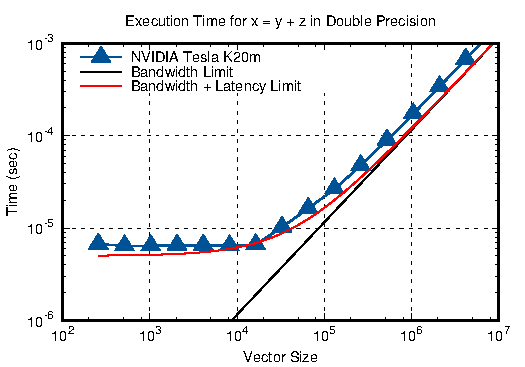
\includegraphics[width=0.75\textwidth]{figures/vector-addition-time-3}}
  
  \only<2>{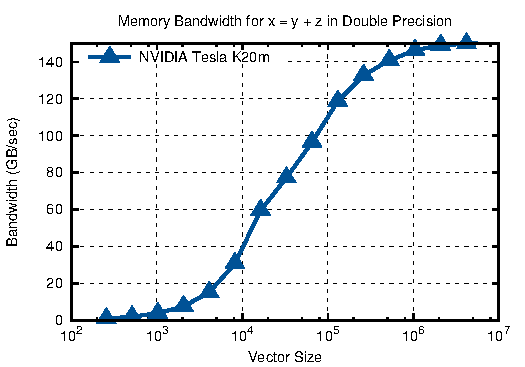
\includegraphics[width=0.75\textwidth]{figures/vector-addition-bw}}
 \end{center}
 
 \end{frame}



